\documentclass[preprint]{article}

\PassOptionsToPackage{numbers,compress}{natbib}

\usepackage[]{neurips_2021}
\usepackage[utf8]{inputenc} 
\usepackage[T1]{fontenc}    
\usepackage{hyperref}       
\usepackage{url}            
\usepackage{booktabs}       
\usepackage{nicefrac}       
\usepackage{microtype}      
\usepackage{amsfonts,amsmath,amssymb}	
\usepackage{mathtools}
\usepackage{lipsum}
\usepackage{atbegshi,picture}
\usepackage[dvipsnames]{xcolor}

\definecolor{linkcolor}{rgb}{0.7752941176470588, 0.22078431372549023, 0.2262745098039215}
\hypersetup{colorlinks=true,
linkcolor=linkcolor,
citecolor=linkcolor,
urlcolor=linkcolor,
linktocpage=true,
pdfproducer=medialab,
}

\title{Inferring dark matter substructure with \\ global astrometry beyond the power spectrum}

\author{
Siddharth Mishra-Sharma \\
The NSF AI Institute for Artificial Intelligence and Fundamental Interactions \\
Massachusetts Institute of Technology \\
Harvard University \\ 
New York University \\
\href{mailto:smsharma@mit.edu}{\texttt{smsharma@mit.edu}} \\
}

% Preprint information
\AtBeginShipoutNext{\AtBeginShipoutUpperLeft{%
  \put(\dimexpr\paperwidth-3.5cm\relax,-1.5cm){MIT-CTP/XXXX}%
}}


\begin{document}
%\preprint{\hfill }

\maketitle

\begin{abstract}
Astrometric lensing has recently emerged as a promising avenue for characterizing the population of dark matter clumps---subhalos---in our Galaxy. Leveraging recent advances in simulation-based inference and neural network architectures, we introduce a novel method to look for global dark matter-induced lensing signatures in astrometric datasets. Our method shows significantly greater sensitivity to a cold dark matter population compared to existing approaches, establishing machine learning as a powerful tool for characterizing dark matter using astrometric data. 
\end{abstract}

\section{Introduction and background}
\label{sec:intro}

Although there exists plenty of evidence for dark matter (DM) on galactic scales and above \emph{e.g.}, observations of galactic rotation curves, the physics of merging galaxy clusters, and the spectrum of fluctuations of the cosmic microwave background, the distribution of DM clumps---subhalos---on sub-galactic scales is less well-understood and remains an active area of cosmological study. This distribution additionally correlates with and may provide clues as to the underlying particle physics nature of dark matter, highlighting its relevance across multiple domains. 

While larger subhalos can be detected and characterized through their association with luminous tracers such as bound stellar populations, subhalos with smaller masses $\lesssim 10^9\,\mathrm M_\odot$ are not generally associated with luminous matter~\cite{Fitts:2016usl,2017MNRAS.467.2019R}, rendering their characterization challenging. Gravitational effects provide one of the few avenues to probe the distribution of these otherwise-invisible subhalos. Gravitational lensing---the bending of light from a background source due to a foreground mass---is one such effect and has been proposed in various incarnations as a probe of dark subhalos. 
 Strong gravitational lensing, for example, has shown promise in probing substructure in galaxies outside of the Milky Way.
 Astrometric lensing has, on the other hand, recently emerged as a powerful probe of the dark matter population in our own Galaxy.

Astrometry refers to the precise measurement of the positions and motions of luminous objects like stars and other galaxies. Gravitational lensing of these background objects by a moving foreground mass, such as a dark matter subhalo, can imprint a characteristic pattern of motions on the measured kinematics (angular velocities and/or accelerations) of these objects. Refs.~\cite{VanTilburg:2018ykj,Mondino:2020rkn} introduced several methods for extracting this signature with the aim of characterizing the subhalo population in our Galaxy, including those based on computing convolutions of the expected lensing signal and detecting local kinematic outliers. Ref.~\cite{Mishra-Sharma:2020ynk} further proposed using the angular power spectrum of the astrometric field as an observable to infer the global properties of a dark matter population.  % \cite{Mondino:2020rkn}

Astrometric datasets are inherently high-dimensional, consisting of positions and kinematics of potentially millions of objects. Especially when the signal consists of the collective imprint of a large number of subhalos, characterizing their population properties involves marginalizing over all possible configurations of subhalos, rendering the likelihood intractable and necessitating a reduction to data summaries like the power spectrum. While shown to be effective, such simplification can result in significant loss of information when the signal is non-Gaussian in nature. Systematic effects such as the existence of large-scale power expressed in the low-dimensional summary domain can further inhibit signal sensitivity. 

The dawn of the era of precision astrometry, with the \emph{Gaia} satellite having delivered the most precise astrometric dataset to-date~\cite{2016A&A...595A...1G,2018A&A...616A...1G,2018A&A...616A...2L} and surveys including the Square Kilometer Array (SKA)~\cite{Fomalont:2004hr,Jarvis:2015tqa} and Roman Space Telescope~\cite{2019JATIS...5d4005W} set to achieve further leaps in sensitivity, calls for methods that can extract more information from these datasets than is possible using existing techniques. In this paper we introduce a method that leverages recent advances in simulation-based inference %and neural network architectures 
in order to characterized the subhalo population in our Galaxy using astrometric data.

\section{Model and inference}
\label{sec:model}

\begin{figure}[!htbp]
\centering
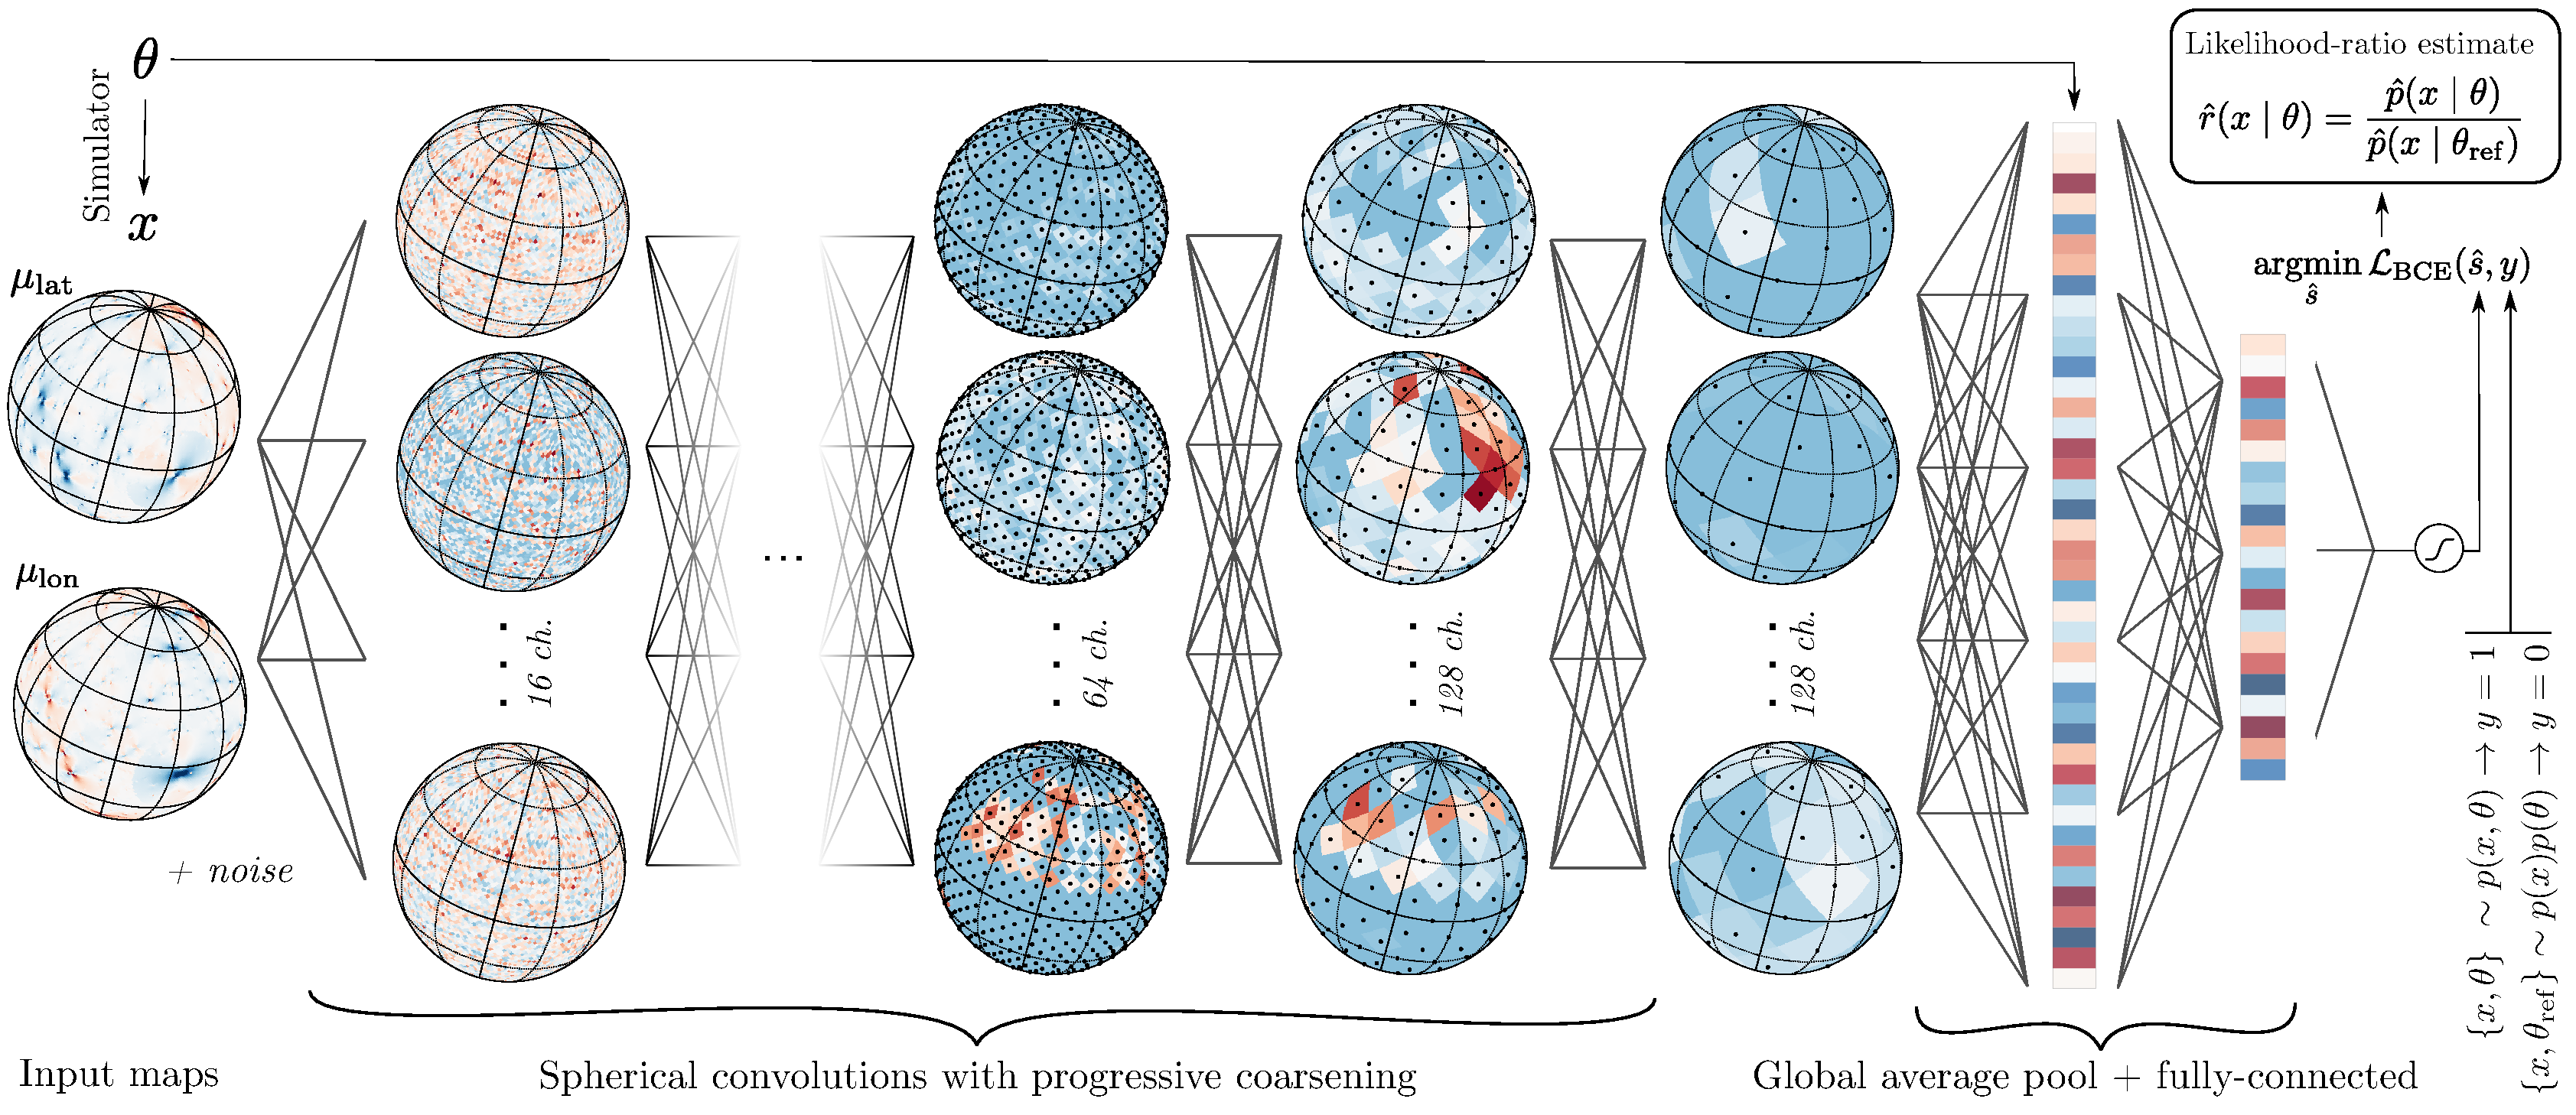
\includegraphics[width=0.98\textwidth]{figures/drawing.pdf}
\caption{An illustration of the method and neural network architecture used in this work.}
\label{fig:model}
\end{figure}

\paragraph{The forward model} We consider a population of Navarro-Frenk-White (NFW)~\cite{Navarro:1995iw} subhalos following a power-law mass function, $\mathrm dn / \mathrm dm \propto m^\alpha$, with slope $\alpha = -1.9$ as expected if the population is sourced from nearly scale-invariant primordial fluctuations in the canonical $\Lambda$ Cold Dark Matter ($\Lambda$CDM) scenario. 
Subhalos between $10^7$--$10^{10}\,\mathrm{M}_\odot$ are simulated, considering the influence of lighter subhalos to be too small to be discernable.
The subhalo fraction $f_\mathrm{sub}$, quantifying the expected fraction of the mass the Milky Way mass contributed by subhalos in the range $10^{-6}$--$10^{10}\,\mathrm{M}_\odot$, is taken to be the parameter of interest. The spatial distribution of subhalos is modeled using results from the Aquarius simulation, following Refs.~\cite{Hutten:2016jko,Springel:2008cc}, which also motivates the benchmark test parameter point containing 150 subhalos in expectation between $10^{8}$--$10^{10}\,\mathrm{M}_\odot$, corresponding to $f_\mathrm{sub} \simeq 0.2$.

Our datasets consist of the 2-dimensional angular velocity map on the celestial sphere of quasi-stellar objects (QSOs), also known as quasars which, owing to their large distances from us, are expected to have small intrinsic angular velocities. 
Given a subhalo lens with velocity $\mathbf{v}_{l}$, the expected induced velocity for a quasar at impact parameter $\mathbf{b}$ is given by~\cite{VanTilburg:2018ykj,Mishra-Sharma:2020ynk}
\begin{equation}
    \boldsymbol{\mu}(\mathbf{b})=4 G_{\mathrm{N}}\left\{\frac{M(b)}{b^{2}}\left[2 \hat{\mathbf{b}}\left(\hat{\mathbf{b}} \cdot \mathbf{v}_{l}\right)-\mathbf{v}_{l}\right]-\frac{M^{\prime}(b)}{b} \hat{\mathbf{b}}\left(\hat{\mathbf{b}} \cdot \mathbf{v}_{l}\right)\right\}
\end{equation}
where $M(b)$ and $M^{\prime}(b)$ are the projected mass and its gradient. An example of the induced velocity signal on part of the celestial sphere, projected along the Galactic  latitudinal and longitudinal directions and exhibiting dipole-like structures, is shown in the leftmost column of Fig.~\ref{fig:model}.

In order to enable comparison with traditional approaches---which are generally not expected to be sensitive to a CDM subhalo population with next-generation astrometric surveys~\cite{VanTilburg:2018ykj,Mishra-Sharma:2020ynk}---we benchmark using an optimistic observational configuration corresponding to measuring the proper motions of $10^8$ quasars with noise $\sigma_{\mu} = 0.1\,\mu\mathrm{as}\,\mathrm{yr}^{-1}$.

\paragraph{The power spectrum approach} Ref.~\cite{Mishra-Sharma:2020ynk} introduced an approach for extracting the astrometric signal due to a dark matter subhalo population by decomposing the observed map into its angular (vector) power spectrum. The power spectrum is a summary statistic ubiquitous in astrophysics and cosmology and quantifies the amount of correlation contained at different spatial scales. In the case of data on a sphere, the basis of spherical harmonics is often used, and the power spectrum then encodes the correlation structure on different multipoles $\ell$. The power spectrum effectively captures the linear component of the signal and, when the underlying signal is a Gaussian random field, captures \emph{all} of the relevant information contained in the map(s)~\cite{Tegmark:1996qt}.
The expected signal and corresponding sensitivity in the power spectrum domain can be computed analytically using the formalism described in Ref.~\cite{Mishra-Sharma:2020ynk}, which we use here as a comparison point. 

While effective, reduction of the full astrometric map to its power spectrum results in loss of information; this can be seen from the fact that the signal on the leftmost column of Fig.~\ref{fig:model} is far from Gaussian. Furthermore, the existence of systematic correlations on large angular scales due to \emph{e.g.}, biases in calibration of celestial reference frames~\cite{2018A&A...616A..14G} introduces degeneracies with a putative signal and precludes their usage in the present context. This is especially true in the case of \emph{relative} astrometric observations, where systematic variations among observed patches of the sky are present. For these reason multipoles $\ell < 10$ were discarded in Ref.~\cite{Mishra-Sharma:2020ynk}, degrading the projected sensitivity.

\paragraph{Simulation-based inference with parameterized classifiers} Recent advances in machine learning have enabled methods that aim to directly extract information from models defined through high-dimensional simulations; see Ref.~\cite{Cranmer:2019eaq} for a recent review. Here, we make use of parameterized classifiers~\cite{Cranmer:2015bka,Baldi:2016fzo,Brehmer:2018eca,Brehmer:2018hga,Brehmer:2018kdj,Hermans:2019ioj} (previously used in Refs.~\cite{Brehmer:2019jyt,Hermans:2020skz} in the context of inferring DM substructure) in order to directly approximate the likelihood ratios associated with all-sky astrometric maps containing signatures of dark matter. Given a classifier that can distinguish between samples $\{x\} \sim p(x\mid\theta)$ and those from a fixed reference hypothesis $\{x\} \sim p(x\mid\theta_\mathrm{ref})$, the decision function output by the optimal classifier $s(x, \theta) = {p(x\mid\theta)}/{\left(p(x\mid\theta) + p(x\mid\theta_\mathrm{ref})\right)}$ is one-to-one with the likelihood ratio, $r(x\mid \theta) \equiv {p(x\mid\theta)}/{p(x\mid\theta_\mathrm{ref})}  = {s(x, \theta)}/{\left(1 - s(x, \theta)\right)}$, a fact appreciated as the likelihood-ratio trick~\cite{Cranmer:2015bka,mohamed2017learning}. 

The classifier $s(x, \theta)$ in this case is a neural network that can work directly on the high-dimensional data $x$, and is parameterized by $\theta$ by having it included as a feature. In order to improve numerical stability and reduce dependence on the fixed reference hypothesis $\theta_\mathrm{ref}$, we follow Ref.~\cite{Hermans:2019ioj} and train a classifier to distinguish between data-sample pairs $\{x, \theta\} \sim p(x,\theta)$ and those from a product of marginal distributions $\{x, \theta\} \sim p(x)p(\theta)$ (obtained by shuffling samples within a batch) using the binary cross-entropy loss as the optimization objective. 

\paragraph{Extracting information from high-dimensional astrometric datasets} We bin the the velocity maps on a \texttt{HEALPix} grid with resolution parameter \texttt{nside=64}, the value in each pixel then quantifying the average velocity of quasars within that pixel. All inputs are normalized to zero mean and unit standard deviation across the training sample. 

We use \texttt{DeepSphere}~\cite{defferrard2020deepsphere,Perraudin:2018rbt}, a graph-based convolutional neural network tailored to data sampled on a sphere and able to leverage the hierarchical structure of the \texttt{HEALPix} representation. In particular, \texttt{DeepSphere} efficiently performs convolutions in the spectral domain, using a basis of Chebychev polynomials as convolutional kernels~\cite{defferrard2016convolutional}. Starting with 2 input channels representing the two orthogonal (Galactic latitude and longitude) components of the velocity vector, we perform a graph convolution operation, increasing the channel dimension to 16, followed by a batch normalization, ReLU nonlinearity, and coarsening of the representation to resolution \texttt{nside=32} with max pooling (downsampling the representation by a factor of 4). 
Pooling leverages scale separation, preserving important characteristics of the signal across different resolutions. 
Four more such layers are employed, increasing the channel dimension by a factor of 2 at each step until a maximum of 128, with the final map having \texttt{nside=2} corresponding to 48 pixels. At this stage, we average over the spatial dimension in order to encourage rotational invariance~\cite{lin2014network}, outputting 128 features onto which the parameter of interest $f_\mathrm{sub}$ is appended. This is passed through a fully-connected network with (1024, 128) hidden units outputting the classifier decision by finally applying a sigmoidal projection.  % appended in order to parameterize

\bigskip

$10^5$ samples from the forward model were produced. The estimator is trained for up to 50 epochs with early stopping, with a batch size of 64. The \texttt{AdamW} optimizer~\cite{kingma2017adam,loshchilov2019decoupled} is used with initial learning rate $10^{-3}$ and weight decay $10^{-5}$, with learning rate decayed through cosine annealing. Figure~\ref{fig:model} summarizes the neural network architecture and method used in this work.

% LRT~\cite{Cranmer:2015bka}
% AALR~\cite{Hermans:2019ioj}
% SBI~\cite{Cranmer:2019eaq}

\begin{figure}[!htbp]
\centering
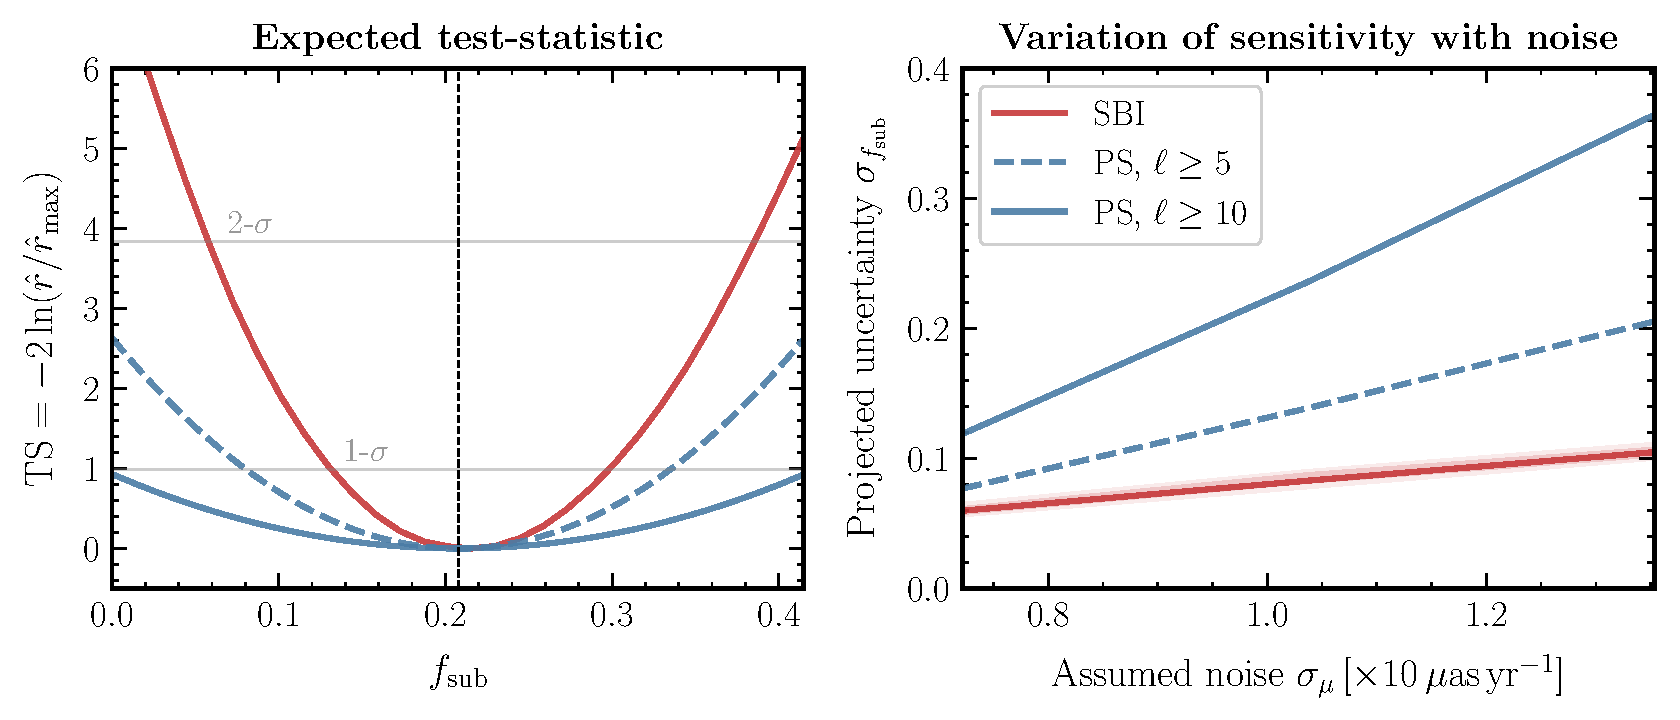
\includegraphics[width=0.98\textwidth]{figures/results}
\caption{\emph{(Left)} The expected test statistic using the machine learning-based method introduced in this work (red line) compared with existing approaches using power spectrum summaries with different multipole thresholds (blue lines). \emph{(Right)} Scaling of the expected sensitivities (given by 1-$\sigma$ uncertainties) with instrumental noise.}
\label{fig:experiment}
\end{figure}
 
% \begin{figure}[!htbp]
% \centering
% 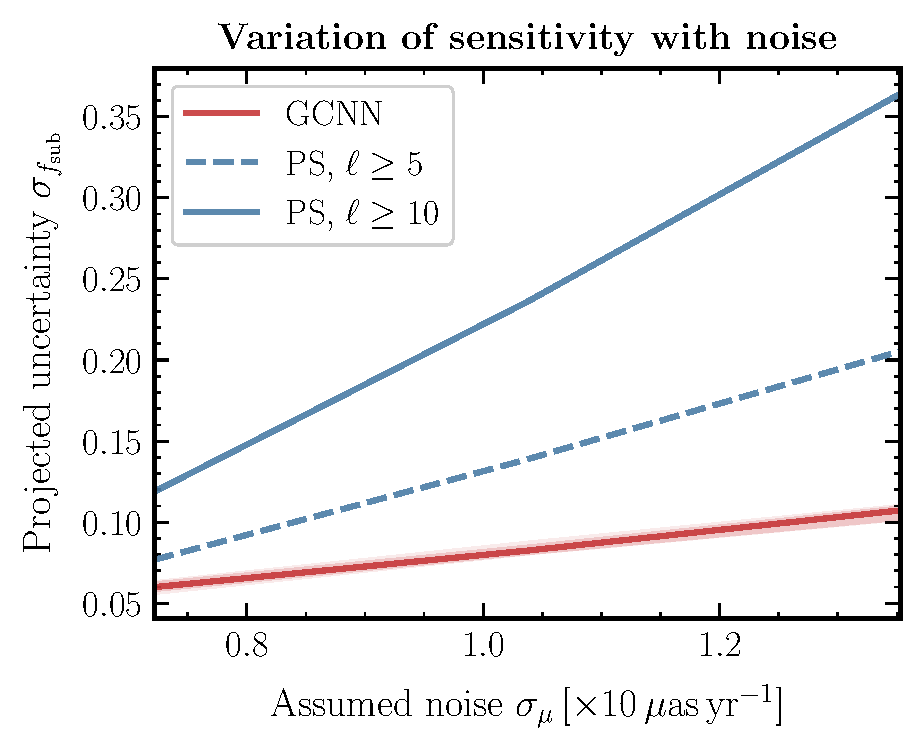
\includegraphics[width=0.49\textwidth]{figures/noise_var}
% \caption{Caption}
% \label{fig:experiment}
% \end{figure}

\section{Experiments on simulated data}
\label{sec:experiments}

The left panel of Fig.~\ref{fig:experiment} shows the expected test statistic (TS), defined as $\mathrm{TS} \equiv -2\ln(\hat r / \hat r_\mathrm{max})$, as a function of substructure fraction $f_\mathrm{sub}$ for the benchmark configuration with $f_\mathrm{sub} \simeq 0.2$. This is obtained by evaluating the trained estimator as a mean over 50 test maps on a uniform grid in $f_\mathrm{sub}$. Corresponding curves using the power spectrum approach are shown in blue, using minimum multipole thresholds of $\ell \geq 5$ (dashed) and $\ell \geq 10$ (solid). Thresholds corresponding to 1- and 2-$\sigma$ significance are shown as the horizontal grey lines. We see that sensitivity gains of over a factor of $\sim 2$ can be expected for this particular benchmark when using the machine learning approach presented here when compared to the traditional power spectrum approach. No significant bias on the central value of the inferred DM abundance relative to the overall uncertainty scale is observed.

The right panel of Fig.~\ref{fig:experiment} shows the scaling of expected sensitivity on substructure fraction $f_\mathrm{sub}$ with assumed noise per quasar, keeping the number of quasars fixed (red, with the line showing the median and shaded dark and light bands corresponding to 1- and 2-$\sigma$ variation, respectively, over 50 test datasets) compared to the power spectrum approach (blue lines). A far more favorable scaling of the machine learning approach is seen compared to the power spectrum approach, suggesting that it is disproportionately advantageous in low signal-to-noise regimes that are generally most relevant for dark matter searches.

\section{Conclusions and outlook}
\label{sec:conclusions}

We have introduced a method to analyze astrometric datasets over large regions of the sky using techniques based on machine learning with the aim of inferring the lensing signature of a dark matter subhalo population. We have shown our method to be significantly more sensitive a CDM subhalo population compared to established methods based on global summary statistics, with more favorable scaling with instrumental noise. Since data collection and reduction is an expensive endeavor, the use of methods that can take advantage of more of the available information can be equated to potentially years of observations, underscoring their importance. Additionally, unlike the power spectrum approach, the current method does not require the construction of a numerically-expensive estimator to account for non-uniform exposure and instrumental noise---these, as well as any other observational effects can be incorporated directly into the forward model. 

The use of architectures that explicitly take the vector nature of the input into account~\cite{esteves2020spinweighted} can further improve the fidelity of the analysis. \cite{Cheng:2020qbx,2021arXiv210709145H,2021arXiv210411244S,2021arXiv210202828M}


We have focused in this work on assessing sensitivity to a CDM-like subhalo population with quasar velocity astrometry, which is within the scope of upcoming radio telescopes like the SKA. Our method can also be applied in a straightforward manner to look for the \emph{acceleration} lensing signal imprinted on Milky Way stars, in particular sourced by a population of more compact subhalos than those expected in CDM. Both of these features are expected to introduce a larger degree of non-Gaussianity than in the signal explored here (as can be seen, \emph{e.g.}, in Fig. 1 of Ref.~\cite{Mishra-Sharma:2020ynk}). Such analyses using Milky Way stellar accelerations is within purview of the upcoming Roman exoplanet microlensing survey~\cite{Pardo:2021uzy} as well as future \emph{Gaia} data releases, and a machine learning approach could provide significant sensitivity gains over existing methods.

Astrometric lensing has been established as a promising way to characterize the Galactic dark matter population, with theoretical progress in recent years going in step with advances on the observational front. While this work is a first attempt at bringing principled machine learning techniques to this field, with the availability of increasingly complex datasets we expect machine learning to be an important general-purpose tool for future astrometric dark matter searches.

Code used for reproducing the results presented in this paper is available at \url{https://github.com/smsharma/global-astrometry-sbi}. 

\begin{ack}
SM warmly thanks Cristina Mondino and Ken Van Tilburg for helpful conversations and comments on the draft. SM benefitted from the hospitality of the Center for Computational Astrophysics at the Flatiron Institute while this work was being performed. 
This work was performed in part at the Aspen Center for Physics, which is supported by National Science Foundation grant PHY-1607611.
The participation of SM at the Aspen Center for Physics was supported by the Simons Foundation.
SM is supported by the NSF CAREER grant PHY-1554858, NSF grants PHY-1620727 and PHY-1915409, and the Simons Foundation. 
This work is supported by the National Science Foundation under Cooperative Agreement PHY-2019786 (The NSF AI Institute for Artificial Intelligence and Fundamental Interactions, \url{http://iaifi.org/}).
This material is based upon work supported by the U.S. Department of Energy, Office of Science, Office of High Energy Physics of U.S. Department of Energy under grant Contract Number DE-SC0012567.
This work made use of the NYU IT High Performance Computing resources, services, and staff expertise. 
This research has made use of NASA's Astrophysics Data System. 

This research made use of the Astropy~\cite{Robitaille:2013mpa,Price-Whelan:2018hus},
Healpy~\cite{Gorski:2004by,Zonca2019},
IPython~\cite{PER-GRA:2007},
Jupyter~\cite{Kluyver2016JupyterN},
Matplotlib~\cite{Hunter:2007},
MLflow~\cite{chen2020developments},
NumPy~\cite{harris_array_2020},
PyGSP~\cite{michael_defferrard_2017_1003158},
PyTorch~\cite{NEURIPS2019_9015},
PyTorch Geometric~\cite{Fey/Lenssen/2019}, 
PyTorch Lightning~\cite{william_falcon_2020_3828935},
sbi~\cite{tejero-cantero2020sbi},
SciPy~\cite{2020SciPy-NMeth}, and
Seaborn~\cite{michael_waskom_2017_883859}
software packages.
We acknowledge the use of the implementation of the \texttt{DeepSphere} graph convolutional layer and code used to produce elements of Fig.~\ref{fig:model} from the code repository associated with Ref.~\cite{defferrard2020deepsphere}.\footnote{\url{https://github.com/deepsphere/deepsphere-pytorch}}
\end{ack}

\bibliographystyle{apsrev4-1-mod}

{
\small
\bibliography{astrometry-sbi}
}

% %%%%%%%%%%%%%%%%%%%%%%%%%%%%%%%%%%%%%%%%%%%%%%%%%%%%%%%%%%%%
% \section*{Checklist}

% \begin{enumerate}

% \item For all authors...
% \begin{enumerate}
%   \item Do the main claims made in the abstract and introduction accurately reflect the paper's contributions and scope?
%     \answerYes{}
%   \item Did you describe the limitations of your work?
%     \answerYes{See Sec.~\ref{sec:conclusions}}
%   \item Did you discuss any potential negative societal impacts of your work?
%     \answerNA{Potential negative societal impacts were considered, and we believe this work does not present any issues in this regard.}
%   \item Have you read the ethics review guidelines and ensured that your paper conforms to them?
%     \answerYes{}
% \end{enumerate}

% \item If you are including theoretical results...
% \begin{enumerate}
%   \item Did you state the full set of assumptions of all theoretical results?
%     \answerNA{No theoretical results were obtained in this work.}
% 	\item Did you include complete proofs of all theoretical results?
%     \answerNA{}
% \end{enumerate}

% \item If you ran experiments...
% \begin{enumerate}
%   \item Did you include the code, data, and instructions needed to reproduce the main experimental results (either in the supplemental material or as a URL)?
%     \answerYes{The code repository associated with this paper and needed to reproduce all the results is linked in Sec.~\ref{sec:conclusions}.}
%   \item Did you specify all the training details (e.g., data splits, hyperparameters, how they were chosen)?
%     \answerYes{These are described in Sec.~\ref{sec:experiments}.}
% 	\item Did you report error bars (e.g., with respect to the random seed after running experiments multiple times)?
%     \answerYes{The main results in Fig.~\ref{fig:experiment} show the expectation evaluated over multiple test datasets. The right panel specifically shows the error bars associated with running over different trials.}
% 	\item Did you include the total amount of compute and the type of resources used (e.g., type of GPUs, internal cluster, or cloud provider)?
%     \answerNo{Due to space constraints limiting the total length of the extended abstract to 4 pages, this information will be included in the camera-ready version of the paper.}
% \end{enumerate}

% \item If you are using existing assets (e.g., code, data, models) or curating/releasing new assets...
% \begin{enumerate}
%   \item If your work uses existing assets, did you cite the creators?
%     \answerYes{All code used for this project is cited in the Acknowledgments section, which is redacted during blind review. Code citations will be reinstated for the camera-ready version of the paper.} 
%   \item Did you mention the license of the assets?
%     \answerNA{Licenses are mentioned in the links associated with individual code packages.}
%   \item Did you include any new assets either in the supplemental material or as a URL?
%     \answerNA{No new assets (excluding the code used to reproduced the experiments) were produced in this work.}
%   \item Did you discuss whether and how consent was obtained from people whose data you're using/curating?
%     \answerNA{}
%   \item Did you discuss whether the data you are using/curating contains personally identifiable information or offensive content?
%     \answerNA{No personal information is included in the assets utilized in this paper.}
% \end{enumerate}

% \item If you used crowdsourcing or conducted research with human subjects...
% \begin{enumerate}
%   \item Did you include the full text of instructions given to participants and screenshots, if applicable?
%     \answerNA{}
%   \item Did you describe any potential participant risks, with links to Institutional Review Board (IRB) approvals, if applicable?
%     \answerNA{}
%   \item Did you include the estimated hourly wage paid to participants and the total amount spent on participant compensation?
%     \answerNA{}
% \end{enumerate}

% \end{enumerate}

%%%%%%%%%%%%%%%%%%%%%%%%%%%%%%%%%%%%%%%%%%%%%%%%%%%%%%%%%%%%

\end{document}